\documentclass[12pt]{report}
\usepackage{amssymb}
\usepackage{multicol}
\usepackage{graphicx}
\usepackage{subfigure}
\usepackage{verbatim}
\usepackage[letterpaper,left=1cm,right=2cm, top=1.5cm,
bottom=1.5cm,head=0cm,foot=1cm]{geometry}

\parindent=0in


\newcommand{\m}{\mbox{ m }}
\newcommand{\kg}{\mbox{ kg }}
\newcommand{\s}{\mbox{ s }}
\newcommand{\ke}{\mbox{\small KE}}
\newcommand{\pe}{\mbox{\small PE}}


\newcommand{ \probDir}[1]{{ \bf\small #1 \mbox{  }}}

\newcommand{ \breakList}{\setcounter{saveenum}{\value{enumi}} \end{enumerate}}
\newcommand{ \contList}{\begin{enumerate} \setcounter{enumi}{\value{saveenum}}}

\newcounter{saveenum}

\def \wspace{5cm}

%%%%%%%%%%%%%%%%%%%%%%%%%%%%%%%%%%%%%%%%%
\begin{document}

{\bf{Honors Physics} \hfill {Quiz 4: Forces and Friction} \hfill {Mr. Kelley}} \\ \\
%%%%%%%%%%
\mbox{} \hfill $\sum F=ma$ \hfill $F_f=\mu F_\bot$ \hfill \mbox{}

\begin{enumerate}
\item A mass of 25 kg is hanging in the center of a clothesline.
\begin{enumerate}
\item What is the force of gravity on the mass?\\
\item What is the tension in each part of the line?\\
\end{enumerate}
\vspace{1cm}

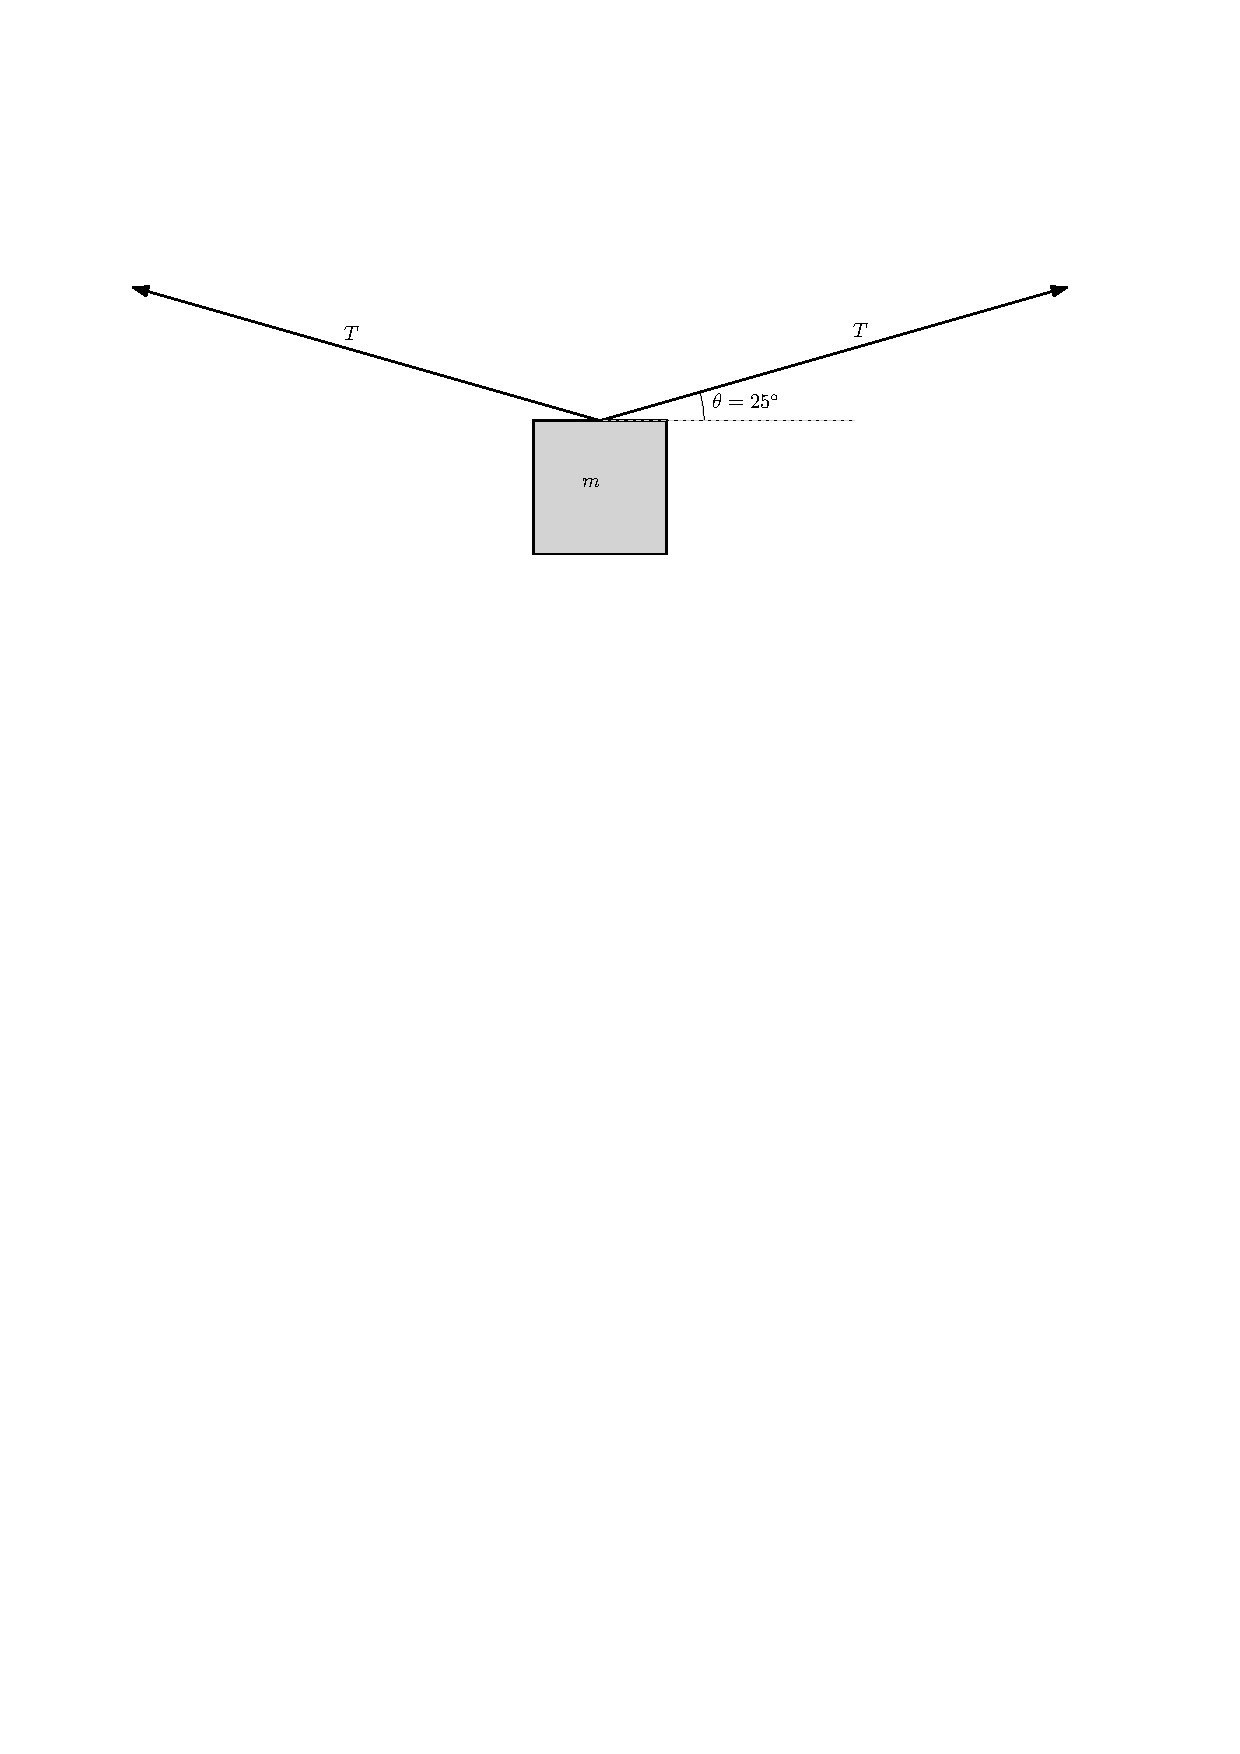
\includegraphics{massClothesline} 

\vspace{4cm}

%\item 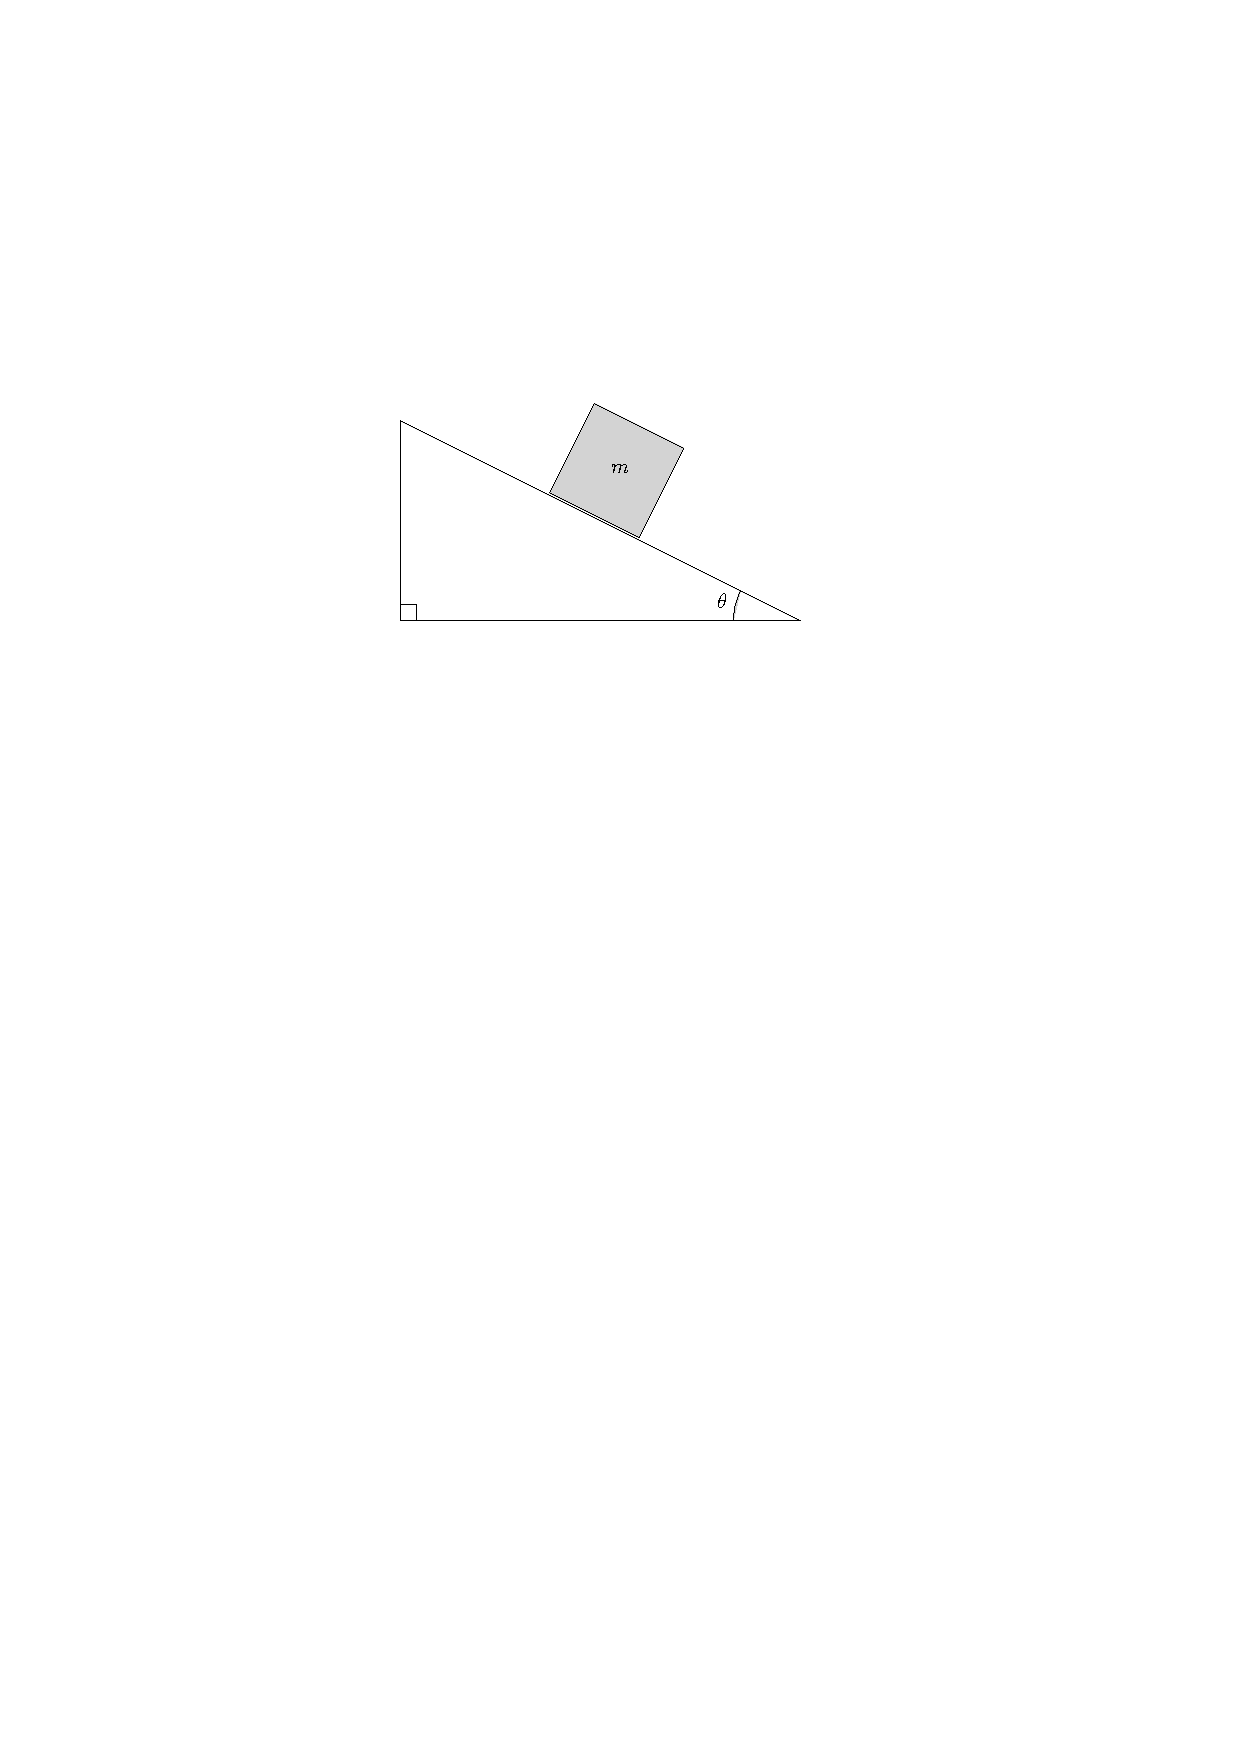
\includegraphics{inclinedPlane}
\item Consider the following frictionless inclined plane and pulley system.  If $\theta = 28^\circ$ and each mass is 15 kg, what is the acceleration of the system?  (Be sure to include direction)

\vspace{1cm}

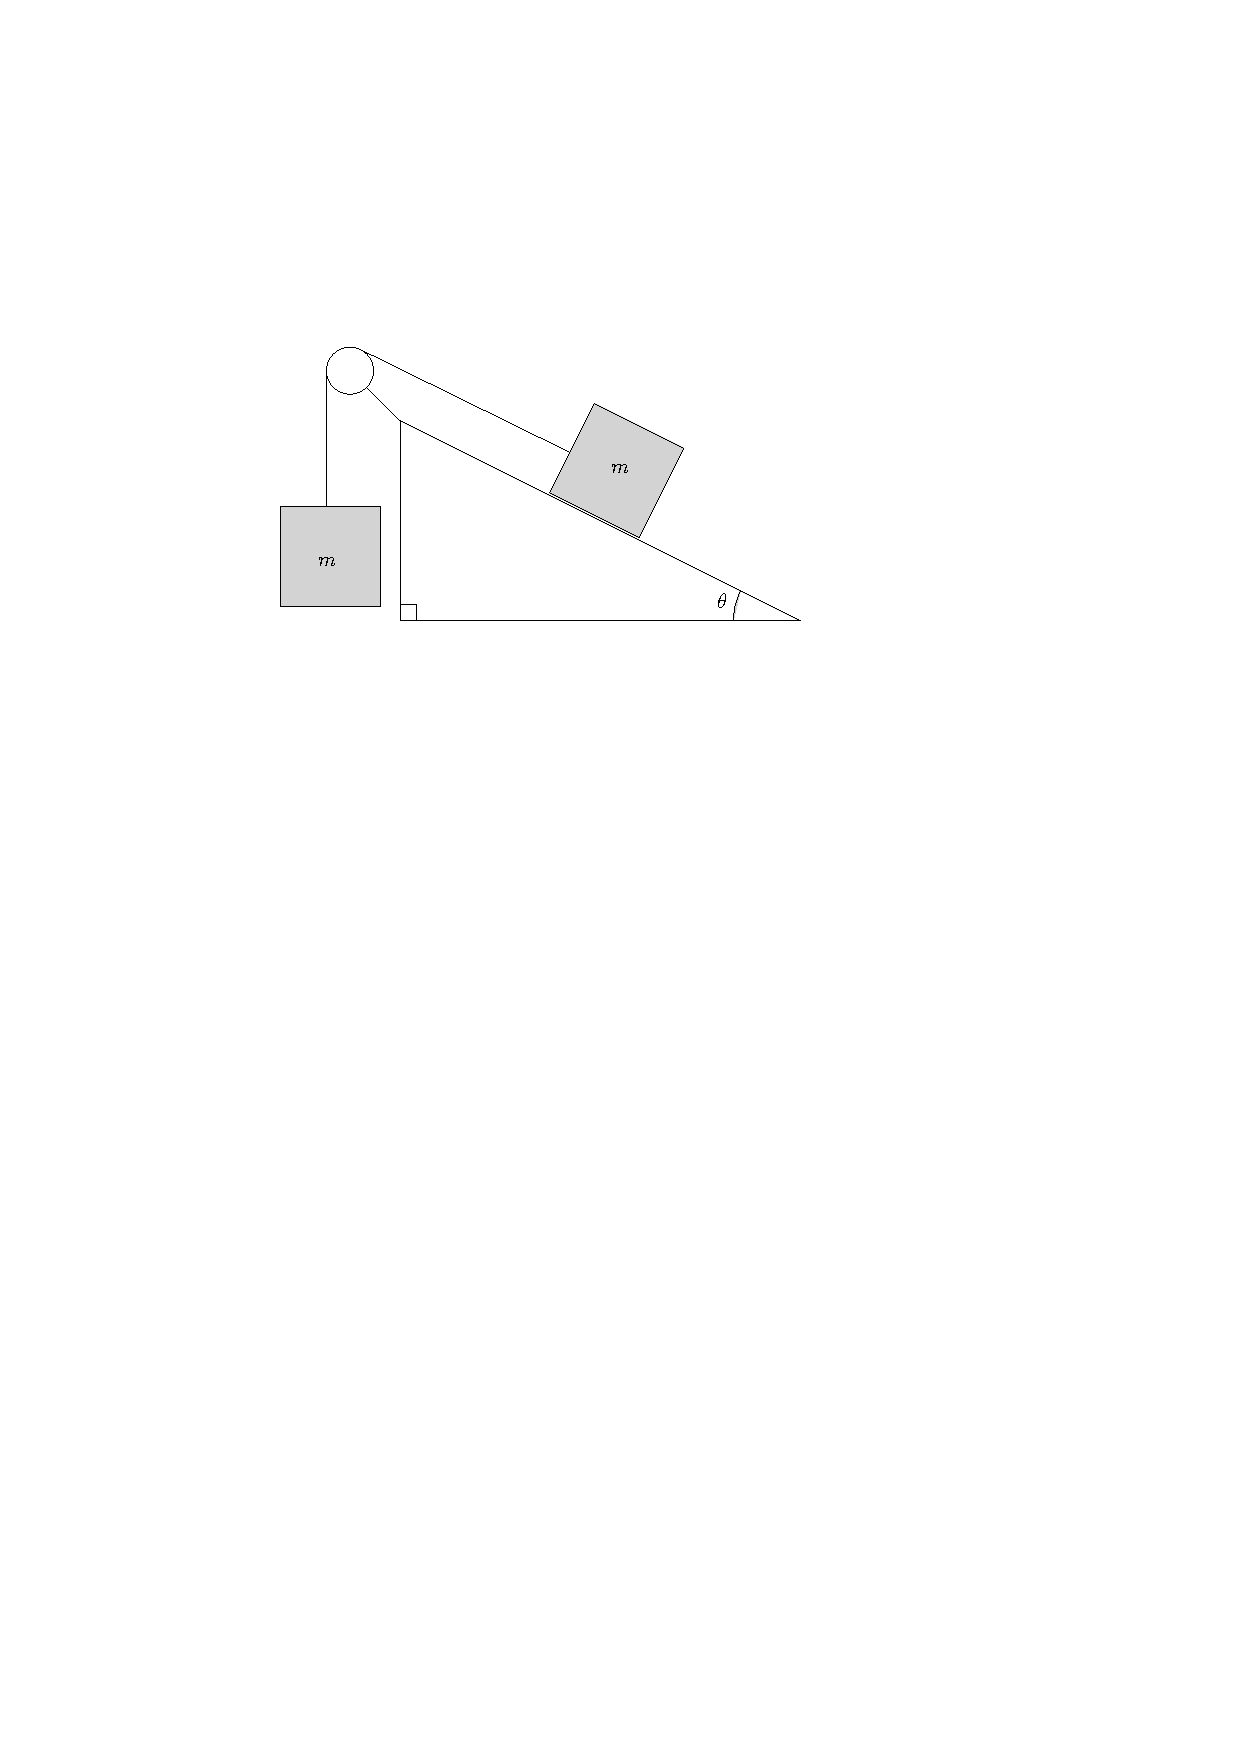
\includegraphics{inclinedPulley} \\
\pagebreak
%%%%%%%
\item A mass is being dragged by a force of 24 N at an angle $\theta = 20^\circ$, and the coefficient of friction between the two surfaces is 0.30 \\
\mbox{} \hfill 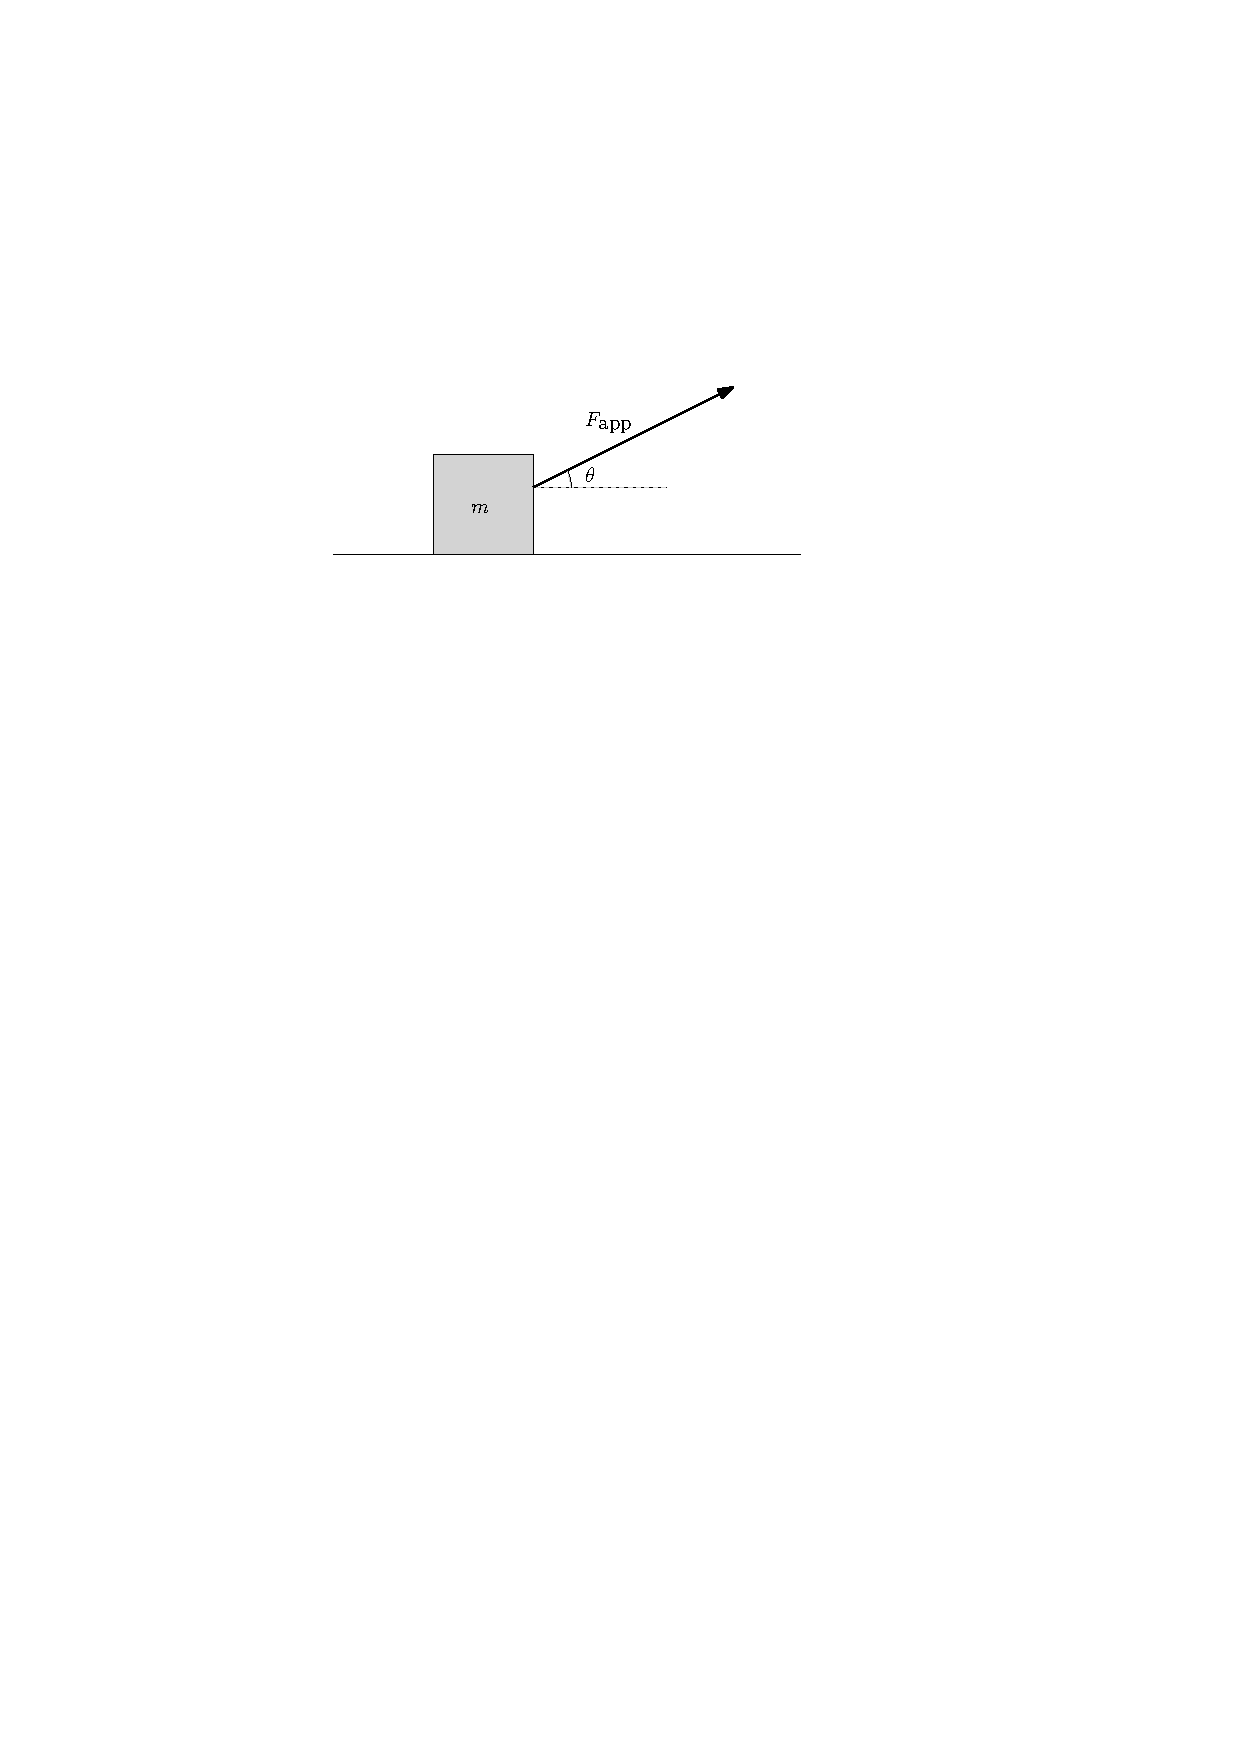
\includegraphics{boxAngle} \hfill \mbox{}
\begin{itemize}
\item What is the normal force on the mass?
\vspace{4cm}
\item What is the acceleration of the mass?
\vspace{5cm}
\end{itemize}




\item Find the expression for the acceleration of this system given that the coefficient of friction is $\mu$ \\

\vspace{2cm}
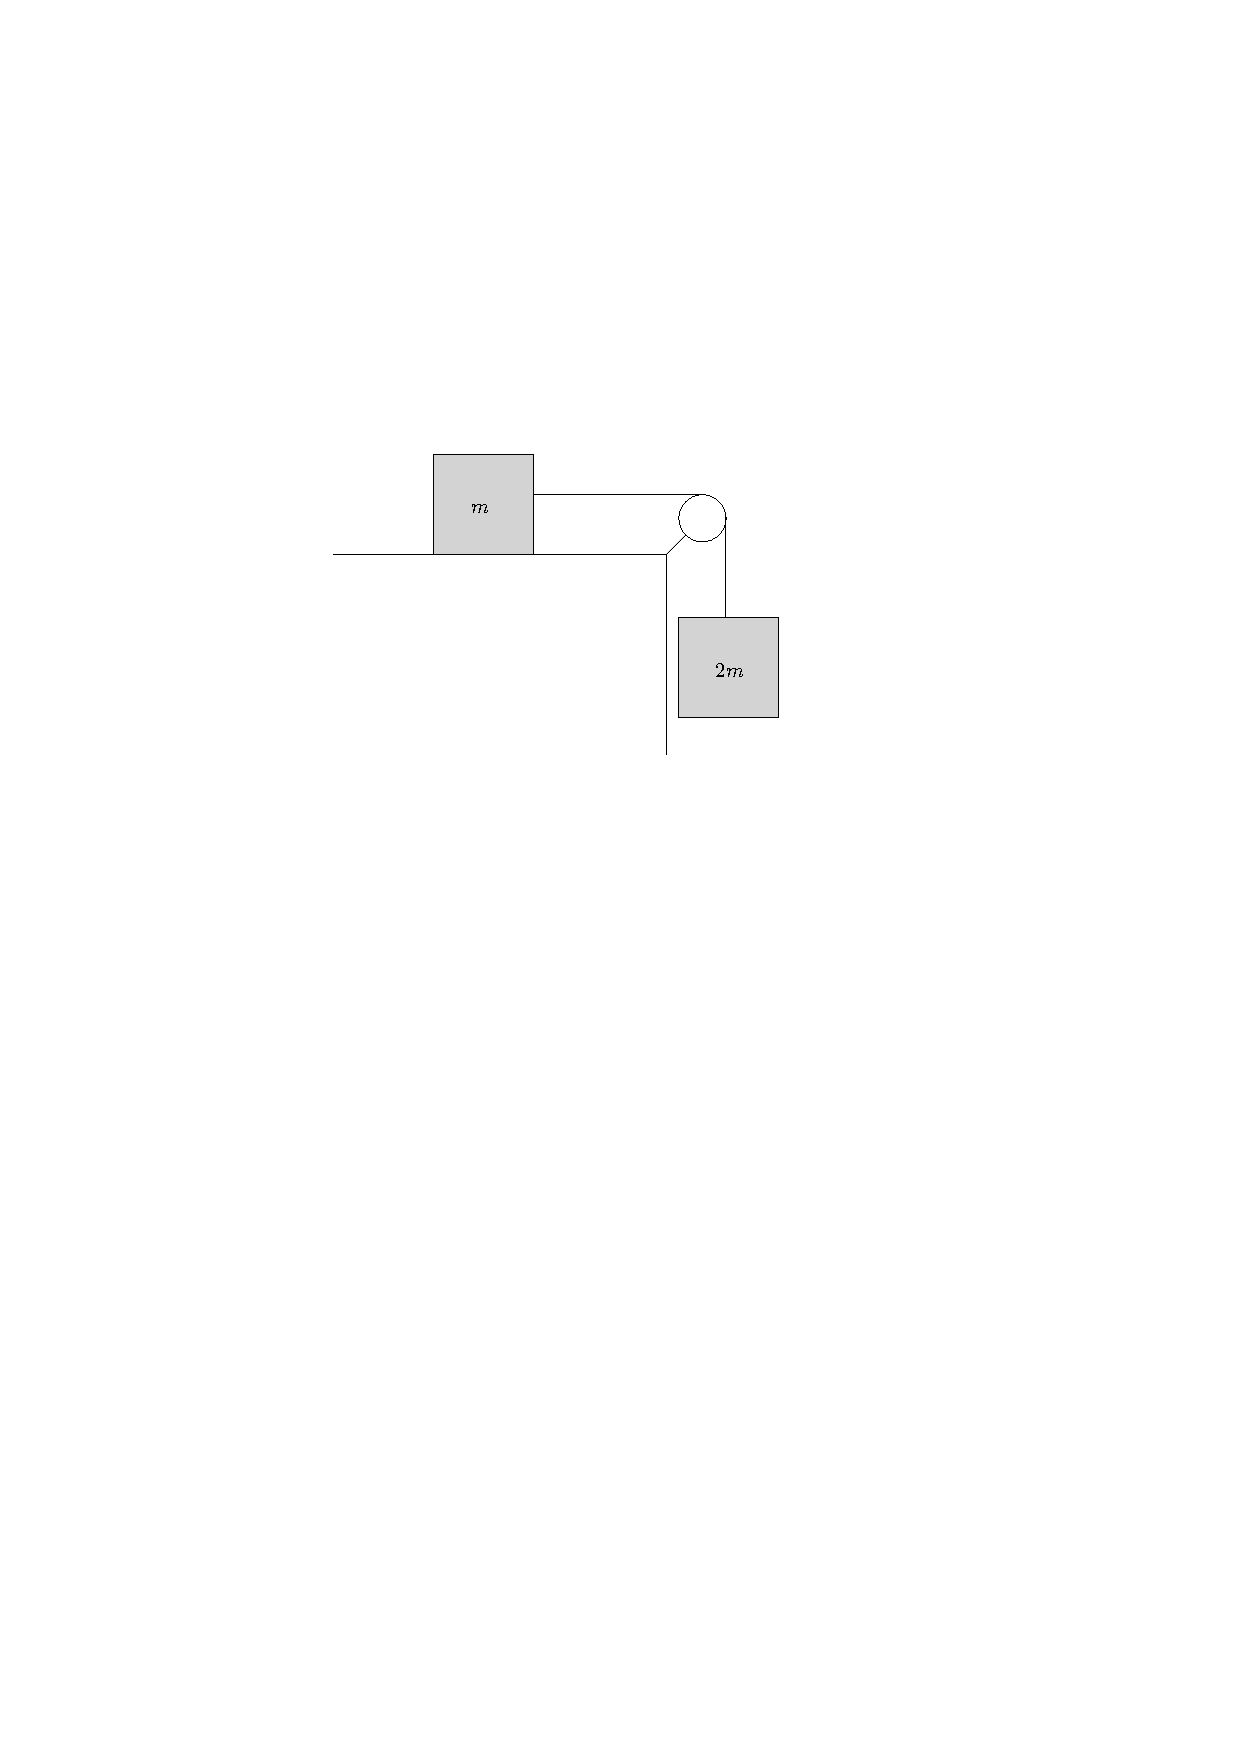
\includegraphics{flatMassPulley}

\vfill
%%%%
\end{enumerate}




\end{document}